
\documentclass{beamer}

\usepackage{xcolor}
\usepackage{color}
\usepackage{graphicx}
\def\xcolorversion{2.00}
\def\xkeyvalversion{1.8}
\setbeamersize{text margin left=0pt,text margin right=0pt}

\makeatletter
\newcommand*\bigcdot{\mathpalette\bigcdot@{.9}}
\newcommand*\bigcdot@[2]{\mathbin{\vcenter{\hbox{\scalebox{#2}{$\m@th#1\bullet$}}}}}
\makeatother

\usepackage{TIKZ_Macra}
\usepackage{xparse}
\usepackage[utf8]{inputenc}
\usepackage[T1]{fontenc}

\useinnertheme[shadow=true]{rounded}
\setbeamercolor{block title}{use=structure,fg=structure.fg,bg=structure.fg!30!bg}
\setbeamercolor{block body}{parent=normal text,use=block title,bg=block title.bg!50!bg}
\setbeamercolor{block title example}{use=example text,fg=example text.fg,bg=example text.fg!30!bg}
\setbeamercolor{block body example}{parent=normal text,use=block title example,bg=block title example.bg!50!bg}

\usepackage[most]{tcolorbox}
\usepackage{lmodern}
\usepackage{mathtools}
\usepackage{amsfonts}
\usepackage{amssymb}
\usepackage{latexsym}
\usepackage{hyperref}
\usepackage{changepage}

\newtcbox{\mybox}{blank, on line, opacitytext=0.5}

\usepackage{Moje_makra}
\usepackage{Moje_Zmienne}
\usepackage{Zbiory_i_konfiguracje}
\usepackage{Complexity}
\usepackage{Sieci}

\newcommand{\Tr}{\mathsf{Tr}}
\newcommand{\Runs}{\mathsf{Runs}}
\newcommand{\PreA}{\mathsf{Pre}}
\newcommand{\PostA}{\mathsf{Post}}
\newcommand{\Part}{\mathcal{P}}
\newcommand{\Blocks}{\mathsf{Blocks}}
\newcommand{\Sat}{\mathsf{Sat}}
\newcommand{\true}{\mathsf{true}}
\newcommand{\false}{\mathsf{false}}
\newcommand{\Act}{\Sigma}
\newcommand{\AP}{\AProp}
\newcommand{\impl}{\mathsf{Impl}}
\newcommand{\absys}{\mathsf{Abs}}
\newcommand{\depth}{\mathsf{md}}

\begin{document}

\begin{frame}[fragile]{}
\Margines{
\begin{center}
  {\huge Theory of Concurrency}\medskip

  {\large Lecture 3b: Computing bisimulation}\medskip

  Partition refinement algorithm\medskip

  Piotr Hofman
\end{center}
}
\end{frame}


\begin{frame}{Goal}
\Margines{
\begin{block}{Input}
A finite labelled transition system
\[
  T=(S,I,\Sigma,\to).
\]
\end{block}

\begin{block}{Output}
The bisimulation equivalence classes of states.
\end{block}

\begin{block}{Why this is useful}
The quotient transition system is smaller and satisfies the same branching-time properties as the original system.
\end{block}
}
\end{frame}

\begin{frame}{Bisimulation as a fixed point}
\Margines{
\begin{block}{Approximants}
Let
\[
  B_0=S\times S.
\]
For \(i\geq 0\), define \((s,t)\in B_{i+1}\) iff, for every \(a\in\Sigma\):
\begin{itemize}
  \item if \(s\xrightarrow{a}s'\), then there exists \(t\xrightarrow{a}t'\) with \((s',t')\in B_i\),
  \item if \(t\xrightarrow{a}t'\), then there exists \(s\xrightarrow{a}s'\) with \((s',t')\in B_i\).
\end{itemize}
\end{block}

\[
  B_0\supseteq B_1\supseteq B_2\supseteq\cdots
\]

For finite systems the sequence stabilizes, and the limit is bisimilarity.
}
\end{frame}

\begin{frame}{From relations to partitions}
\Margines{
\begin{block}{Equivalence relation as a partition}
If \(B\) is an equivalence relation on \(S\), it partitions \(S\) into equivalence classes.
\end{block}

\begin{block}{Initial partition}
For Kripke structures, start by separating states with different labels:
\[
  s\equiv_0 t
  \quad\Longleftrightarrow\quad
  L(s)=L(t).
\]
For plain LTSs without state labels, one may start with one block \(S\).
\end{block}

\begin{block}{Refinement idea}
Repeatedly split blocks until all states in one block have the same observable one-step behaviour with respect to the current partition.
\end{block}
}
\end{frame}

\begin{frame}{Predecessor sets}
\Margines{
For a block \(C\subseteq S\) and an action \(a\in\Sigma\), define
\[
  \PreA_a(C)=\{s\in S : \exists t\in C\; s\xrightarrow{a}t\}.
\]

\begin{block}{Meaning}
\(\PreA_a(C)\) is the set of states that can reach the block \(C\) by an \(a\)-transition.
\end{block}

\begin{block}{When does \(C\) split a block \(B\)?}
The block \(B\) is split by \((a,C)\) if
\[
  B\cap \PreA_a(C)\neq\emptyset
  \quad\text{and}\quad
  B\setminus \PreA_a(C)\neq\emptyset.
\]
\end{block}
}
\end{frame}

\begin{frame}{Split operation}
\Margines{
\begin{block}{Definition}
Given a partition \(\Part\), a block \(C\in\Part\), and an action \(a\in\Sigma\), replace every block \(B\in\Part\) by the non-empty sets among
\[
  B_1=B\cap \PreA_a(C),
  \qquad
  B_2=B\setminus \PreA_a(C).
\]
\end{block}

\begin{block}{Intuition}
States in \(B_1\) can do an \(a\)-move into \(C\). States in \(B_2\) cannot. Therefore they cannot stay bisimilar.
\end{block}
}
\end{frame}

\begin{frame}{Naive partition refinement algorithm}
\Margines{
\begin{enumerate}
  \item Initialize a partition \(\Part\).
  \item While there exist \(a\in\Sigma\) and blocks \(B,C\in\Part\) such that \(C\) splits \(B\):
  \[
    B := B\cap\PreA_a(C),\quad B\setminus\PreA_a(C).
  \]
  \item Return the final partition.
\end{enumerate}

\begin{block}{Termination}
Every proper split increases the number of blocks. There are at most \(|S|\) blocks.
\end{block}

\begin{block}{Correctness intuition}
At the end, states in one block can match transitions to the same blocks, and therefore the partition defines a bisimulation.
\end{block}
}
\end{frame}

\begin{frame}{Stable partitions}
\Margines{
\begin{block}{Stability}
A partition \(\Part\) is stable if for every \(a\in\Sigma\) and every block \(C\in\Part\), no block \(B\in\Part\) is split by \((a,C)\).
\end{block}

Equivalently, for all blocks \(B,C\) and every \(a\in\Sigma\), either
\[
  B\subseteq \PreA_a(C)
\]
or
\[
  B\cap\PreA_a(C)=\emptyset.
\]

\begin{block}{Theorem}
The coarsest stable refinement of the initial partition is the bisimulation quotient.
\end{block}
}
\end{frame}

\begin{frame}{Correctness: why stable means bisimulation}
\Margines{
Let \(\Part\) be stable. Define
\[
  s\equiv_\Part t
  \quad\Longleftrightarrow\quad
  s,t\text{ are in the same block of }\Part.
\]

\begin{block}{Claim}
\(\equiv_\Part\) is a bisimulation.
\end{block}

\begin{block}{Proof idea}
Assume \(s\equiv_\Part t\) and \(s\xrightarrow{a}s'\). Let \(C\) be the block of \(s'\). Then \(s\in\PreA_a(C)\). By stability, the whole block of \(s\) is contained in \(\PreA_a(C)\). Hence \(t\) also has an \(a\)-successor in \(C\).
\end{block}
}
\end{frame}

\begin{frame}{Example of one split}
\Margines{
\begin{center}
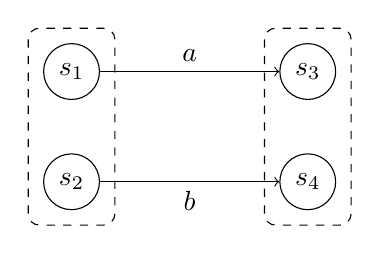
\begin{tikzpicture}[->,node distance=1.7cm]
  \tikzstyle{state}=[circle,draw,minimum size=7mm]
  \node[state] (s1) at (0,0) {$s_1$};
  \node[state] (s2) at (0,-1.4) {$s_2$};
  \node[state] (s3) at (3,0) {$s_3$};
  \node[state] (s4) at (3,-1.4) {$s_4$};
  \draw (s1) -- node[above] {$a$} (s3);
  \draw (s2) -- node[below] {$b$} (s4);
  \draw[dashed,rounded corners] (-0.55,0.55) rectangle (0.55,-1.95);
  \draw[dashed,rounded corners] (2.45,0.55) rectangle (3.55,-1.95);
\end{tikzpicture}
\end{center}

Suppose initially
\[
  \Part=\{\{s_1,s_2\},\{s_3,s_4\}\}.
\]
The block \(C=\{s_3,s_4\}\) and action \(a\) split \(\{s_1,s_2\}\), because only \(s_1\) has an \(a\)-transition into \(C\).

\[
  \{s_1,s_2\}\quad\leadsto\quad \{s_1\},\{s_2\}.
\]
}
\end{frame}

\begin{frame}{Complexity}
\Margines{
\begin{block}{Naive implementation}
The basic refinement algorithm is polynomial and sufficient for understanding the construction.
\end{block}

\begin{block}{Efficient implementation}
With suitable data structures, Paige--Tarjan partition refinement computes bisimulation in time
\[
  O(m\log n),
\]
where \(n=|S|\) and \(m=|\to|\).
\end{block}

\begin{block}{Main idea}
After a split, process the smaller part as a splitter. A state can belong to such a smaller splitter only \(O(\log n)\) times.
\end{block}
}
\end{frame}

\begin{frame}{Summary}
\Margines{
\begin{itemize}
  \item Bisimilarity is the greatest fixed point of the bisimulation conditions.
  \item For finite systems it can be computed by repeated refinement.
  \item A stable partition is exactly a partition into bisimulation classes.
  \item The quotient preserves branching-time properties invariant under bisimulation.
\end{itemize}
}
\end{frame}

\end{document}
